% Fig. 1: causal chain from robot action to robot observation. Redrawn in TikZ 2026-11-04 from the Google-Drawings
% raster "Surgical Robot Causal Chain.png" (kept beside this file). One-column figure: 3.5 in wide, Times (mathptmx),
% all text 9 pt (\small of a 10 pt document). Dashed outline and dashed arrows = not implemented in this work.
% The asterisk on "Contact force" is explained in the caption (computed by the solver, not reported, Sec. IV-D).
% Build (docker, then crop):
%   docker run --rm -v "$PWD":/work -w /work texlive/texlive:latest-medium sh -c \
%     "pdflatex -interaction=nonstopmode fig_causal_chain.tex && pdfcrop --margins 1 fig_causal_chain.pdf fig_causal_chain.pdf"
\documentclass[10pt]{article}
\usepackage{mathptmx}
\usepackage{tikz}
\usetikzlibrary{arrows.meta,positioning,fit,calc}
\pagestyle{empty}
\begin{document}
\small
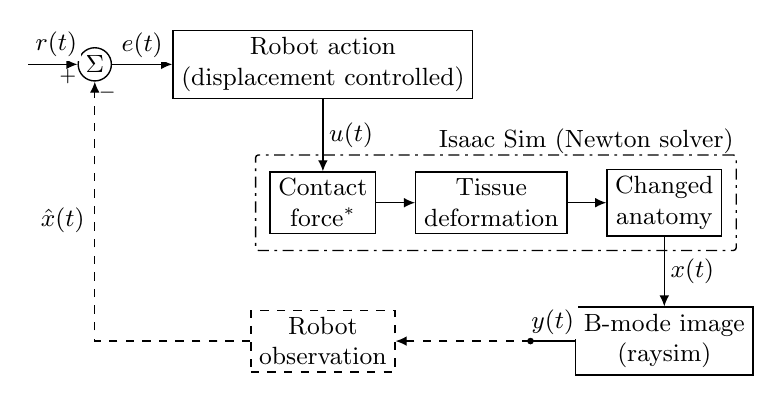
\begin{tikzpicture}[
  x=1pt, y=1pt,
  font=\small,
  box/.style={draw, fill=white, rectangle, align=center, inner xsep=3pt, inner ysep=2.5pt, minimum height=20pt, line width=0.5pt},
  notimpl/.style={box, dashed},
  group/.style={draw, dash pattern=on 4pt off 2pt on 1pt off 2pt, line width=0.5pt, inner sep=5pt, rounded corners=1pt},
  sig/.style={-{Latex[length=4pt,width=3.5pt]}, line width=0.5pt},
  sigd/.style={sig, dashed},
  lab/.style={inner sep=1.5pt, fill=white},
  sum/.style={draw, circle, minimum size=12pt, inner sep=0pt, line width=0.5pt}]

% ---- row 1: reference, summing junction, robot action
\node[sum] (sum) at (26,0) {$\Sigma$};
\node[box, anchor=west] (robot) at (54,0) {Robot action\\(displacement controlled)};
\draw[sig] (2,0) -- (sum.west) node[lab, pos=0.05, above=1pt, anchor=south west] {$r(t)$};
\node[inner sep=0pt] at ($(sum.west)+(-3.5,-4.5)$) {\scriptsize$+$};
\draw[sig] (sum.east) -- (robot.west) node[lab, midway, above=0.5pt] {$e(t)$};

% ---- row 2: the simulator group (contact force -> tissue deformation -> changed anatomy)
\node[box] (cf) at (robot.south |- 0,-50) {Contact\\force$^{*}$};
\node[box, right=14pt of cf] (td) {Tissue\\deformation};
\node[box, right=14pt of td] (ca) {Changed\\anatomy};
\node[group, fit=(cf)(td)(ca), label={[anchor=south east, inner sep=1pt, yshift=-1pt]north east:Isaac Sim (Newton solver)}] (sim) {};
\draw[sig] (robot.south) -- (cf.north) node[lab, midway, right=0.5pt] {$u(t)$};
\draw[sig] (cf.east) -- (td.west);
\draw[sig] (td.east) -- (ca.west);

% ---- row 3: B-mode image (output) and the robot observation (not implemented)
\node[box] (bm) at (ca.south |- 0,-100) {B-mode image\\(raysim)};
\node[notimpl] (obs) at (cf.south |- bm) {Robot\\observation};
\draw[sig] (ca.south) -- (bm.north) node[lab, midway, right=0.5pt] {$x(t)$};
\coordinate (tap) at ($(bm.west)+(-16,0)$);
\draw[line width=0.5pt] (bm.west) -- (tap) node[lab, midway, above=0.5pt] {$y(t)$};
\fill (tap) circle (1.2pt);
\draw[sigd] (tap) -- (obs.east);
% feedback: observation -> state estimate -> summing junction (minus)
\draw[sigd] (obs.west) -- ++(-12,0) -| (sum.south);
\node[lab, anchor=east] at ($(sum.south)+(-2,-50)$) {$\hat{x}(t)$};
\node[inner sep=0pt] at ($(sum.south)+(4.5,-4)$) {\scriptsize$-$};
\end{tikzpicture}
\end{document}
